\documentclass{article}

\usepackage{fancyhdr} % Required for custom headers
\usepackage{lastpage} % Required to determine the last page for the footer
\usepackage{extramarks} % Required for headers and footers
\usepackage[usenames,dvipsnames]{color} % Required for custom colors
\usepackage{graphicx} % Required to insert images
\usepackage{listings} % Required for insertion of code
\usepackage{courier} % Required for the courier font
\usepackage{lipsum} % Used for inserting dummy 'Lorem ipsum' text into the template
\usepackage{hyperref}
\usepackage{multirow}
\usepackage{tabularx}
\usepackage{framed}
\usepackage{longtable}
\usepackage{listings}
\usepackage{subfigure}
\usepackage{afterpage}
\usepackage{amsmath,amssymb}            
\usepackage{rotating}  
\usepackage{fancyhdr}
\usepackage{graphicx}
\usepackage{amsthm}
\usepackage[scriptsize]{caption} 
\hyphenation{a-gen-tiz-za-zio-ne}
% Margins
\topmargin=-0.45in
\evensidemargin=0in
\oddsidemargin=0in
\textwidth=6.5in
\textheight=9.0in
\headsep=0.25in

\linespread{1.1} % Line spacing

\lstset{
  numbers=left,
  stepnumber=5,    
  firstnumber=1,
  numberfirstline=true
}

% Set up the header and footer
\pagestyle{fancy}
\lhead{\hmwkAuthorName} % Top left header
\chead{\hmwkClass\ (\hmwkClassInstructor\ \hmwkClassTime): \hmwkTitle} % Top center head
\rhead{\firstxmark} % Top right header
\lfoot{\lastxmark} % Bottom left footer
\cfoot{} % Bottom center footer
\rfoot{Page\ \thepage\ of\ \protect\pageref{LastPage}} % Bottom right footer
\renewcommand\headrulewidth{0.4pt} % Size of the header rule
\renewcommand\footrulewidth{0.4pt} % Size of the footer rule

\setlength\parindent{0pt} % Removes all indentation from paragraphs

\usepackage{listings}
\usepackage{color}

\definecolor{dkgreen}{rgb}{0,0.6,0}
\definecolor{gray}{rgb}{0.5,0.5,0.5}
\definecolor{mauve}{rgb}{0.58,0,0.82}

\lstset{frame=tb,
  language=Java,
  aboveskip=3mm,
  belowskip=3mm,
  showstringspaces=false,
  columns=flexible,
  basicstyle={\small\ttfamily},
  numbers=none,
  numberstyle=\tiny\color{gray},
  keywordstyle=\color{blue},
  commentstyle=\color{dkgreen},
  stringstyle=\color{mauve},
  breaklines=true,
  breakatwhitespace=true
  tabsize=3
}

%----------------------------------------------------------------------------------------
%	DOCUMENT STRUCTURE COMMANDS
%	Skip this unless you know what you're doing
%----------------------------------------------------------------------------------------

% Header and footer for when a page split occurs within a problem environment
\newcommand{\enterProblemHeader}[1]{
\nobreak\extramarks{#1}{#1 continued on next page\ldots}\nobreak
\nobreak\extramarks{#1 (continued)}{#1 continued on next page\ldots}\nobreak
}

% Header and footer for when a page split occurs between problem environments
\newcommand{\exitProblemHeader}[1]{
\nobreak\extramarks{#1 (continued)}{#1 continued on next page\ldots}\nobreak
\nobreak\extramarks{#1}{}\nobreak
}






%----------------------------------------------------------------------------------------
%	NAME AND CLASS SECTION
%----------------------------------------------------------------------------------------

\newcommand{\hmwkTitle}{Pattern Strutturali e Comportamentali} % Assignment title
\newcommand{\hmwkDueDate}{Venerd\`i,\ Aprile 15,\ 2015} % Due date
\newcommand{\hmwkClass}{Ingegneria del Software 1} % Course/class
\newcommand{\hmwkClassTime}{} % Class/lecture time
\newcommand{\hmwkClassInstructor}{Claudio Menghi, Alessandro Rizzi} % Teacher/lecturer
\newcommand{\hmwkAuthorName}{} % Your name

%----------------------------------------------------------------------------------------
%	TITLE PAGE
%----------------------------------------------------------------------------------------
\newcounter{EsercizioCounter}
 \setcounter{EsercizioCounter}{1}


\newcommand{\Esercizio}[1]{
%\setlength{\fboxsep}{2pt}
\fbox{
   
  \parbox[t][]{\textwidth}{
   \vspace{2ex}
   \textbf{Esercizio \arabic{EsercizioCounter}}: #1
    \vspace{2ex}
    \refstepcounter{EsercizioCounter}
  }
}
}


%----------------------------------------------------------------------------------------

\begin{document}

\maketitle

%----------------------------------------------------------------------------------------
%	TABLE OF CONTENTS
%----------------------------------------------------------------------------------------

%\setcounter{tocdepth}{1} % Uncomment this line if you don't want subsections listed in the ToC

\newpage
\tableofcontents
\newpage



\section{Introduzione}
I problemi incontrati nello sviluppo di grossi progetti software sono spesso ricorrenti e prevedibili
\begin{itemize}
\item I  design pattern sono ``schemi di soluzioni" riutilizzabili
\item  Permettono quindi di non inventare da capo soluzioni ai problemi gi\`a risolti, ma di utilizzare dei ``mattoni" di provata efficacia
\begin{itemize}
\item Un bravo progettista sa riconoscerli, nella documentazione o direttamente nel codice, e utilizzarli per comprendere i programmi scritti da altri
\item forniscono quindi un vocabolario comune che facilita la comunicazione tra progettisti
\end{itemize}
\item Possono rendere la struttura del progetto/codice pi\`u complessa del necessario
\end{itemize}

Un applicazione pu\`o essere suddivisa in tre parti:
\begin{itemize}
\item creazionale: riguarda il processo di creazione degli oggetti
\item strutturale: hanno a che fare con la composizione di classi e oggetti
\item comportamentale: si occupa di come interagiscono gli oggetti
\end{itemize}
Per ognuna di queste parti sono stati identificati dei pattern specifici.  

\subsection{Pattern strutturali}

Si riferiscono a come classi e oggetti sono composti per formare strutture (funzionalit\`a) pi\`u complesse. L'idea \`e quella di aggiungere flessibilit\`a consentendo di comporre le classi a run-time, creando nuove funzionalit\`a

\begin{itemize}
\item \emph{Adapter}: rende un interfaccia conforme ad un altra, fornendo un astrazione comune alle due interfacce. 
\item \emph{Proxy}: consente di creare un placeholder per una altro componente, di cui pu\`o restringere o migliorare le funzionalit\`a.
\item \emph{Decorator}: consente di aggiungere funzionalit\`a all'oggetto dinamicamente.
\end{itemize}






\subsubsection{Adapter/Wrapper}
\begin{framed}
\emph{Converte un interfaccia di una classe in un altra interfaccia che il cliente si aspetta. L'adater permette di utilizzare classi insieme che altrimenti non sarebbero compatibili a causa delle loro interfacce}
\end{framed}


Considerate per esempio un framework che consente di disegnare figure come linee, poligoni, cerchi etc. In genere \`e possibile astrarre un elemento disegnabile utilizzando un \emph{interfaccia} o una \emph{classe} \texttt{Shape}, che fornische dei metodi per disegnare l'elemento e cambiarne le dimensioni. \`E possibile implementare/estendere l'interfaccia/classe \texttt{Shape} specificando i comportamenti per i vari elementi. Tuttavia, per uno di questi componenti potrebbe essere utile utilizzare una libreria esterna. Per esempio immaginiamo di avere una libreria esterna che gestisce i cerchi. Come possiamo utilizzare la classe cerchio all'interno del nostro tool? Ovviamente la classe cerchio conterr\`a dei metodi con nomi differenti rispetto a quelli che abbiamo dichiarato in \texttt{Shape}, inoltre alcuni metodi potrebbero mancare. La soluzione consiste nell'utilizzo del pattern \emph{adapter}. L'adapter converte le funzioalit\`a della classe adattata a quella della classe target e implementa le funzionalit\`a che la classe adattata non fornisce. Per esempio implementa metodi addizionali o controlli che la classe adattata non contiene. Per esempio la libreria che utilizziamo potrebbe non contenere il metodo per ridimenionare gli oggetti contenuto in Shape.

Il pattern adapter va utilizzato quando:
\begin{itemize}
\item volete utilizzare una classe che esiste gi\`a e la sua interfaccia non matcha l'interfaccia richiesta
\item volete creare una classe riusabile che incorpora un insieme di classi che non sono relazioate (per esempio classi che provengono da librerie diverse)
\end{itemize}


\begin{figure}
\centering
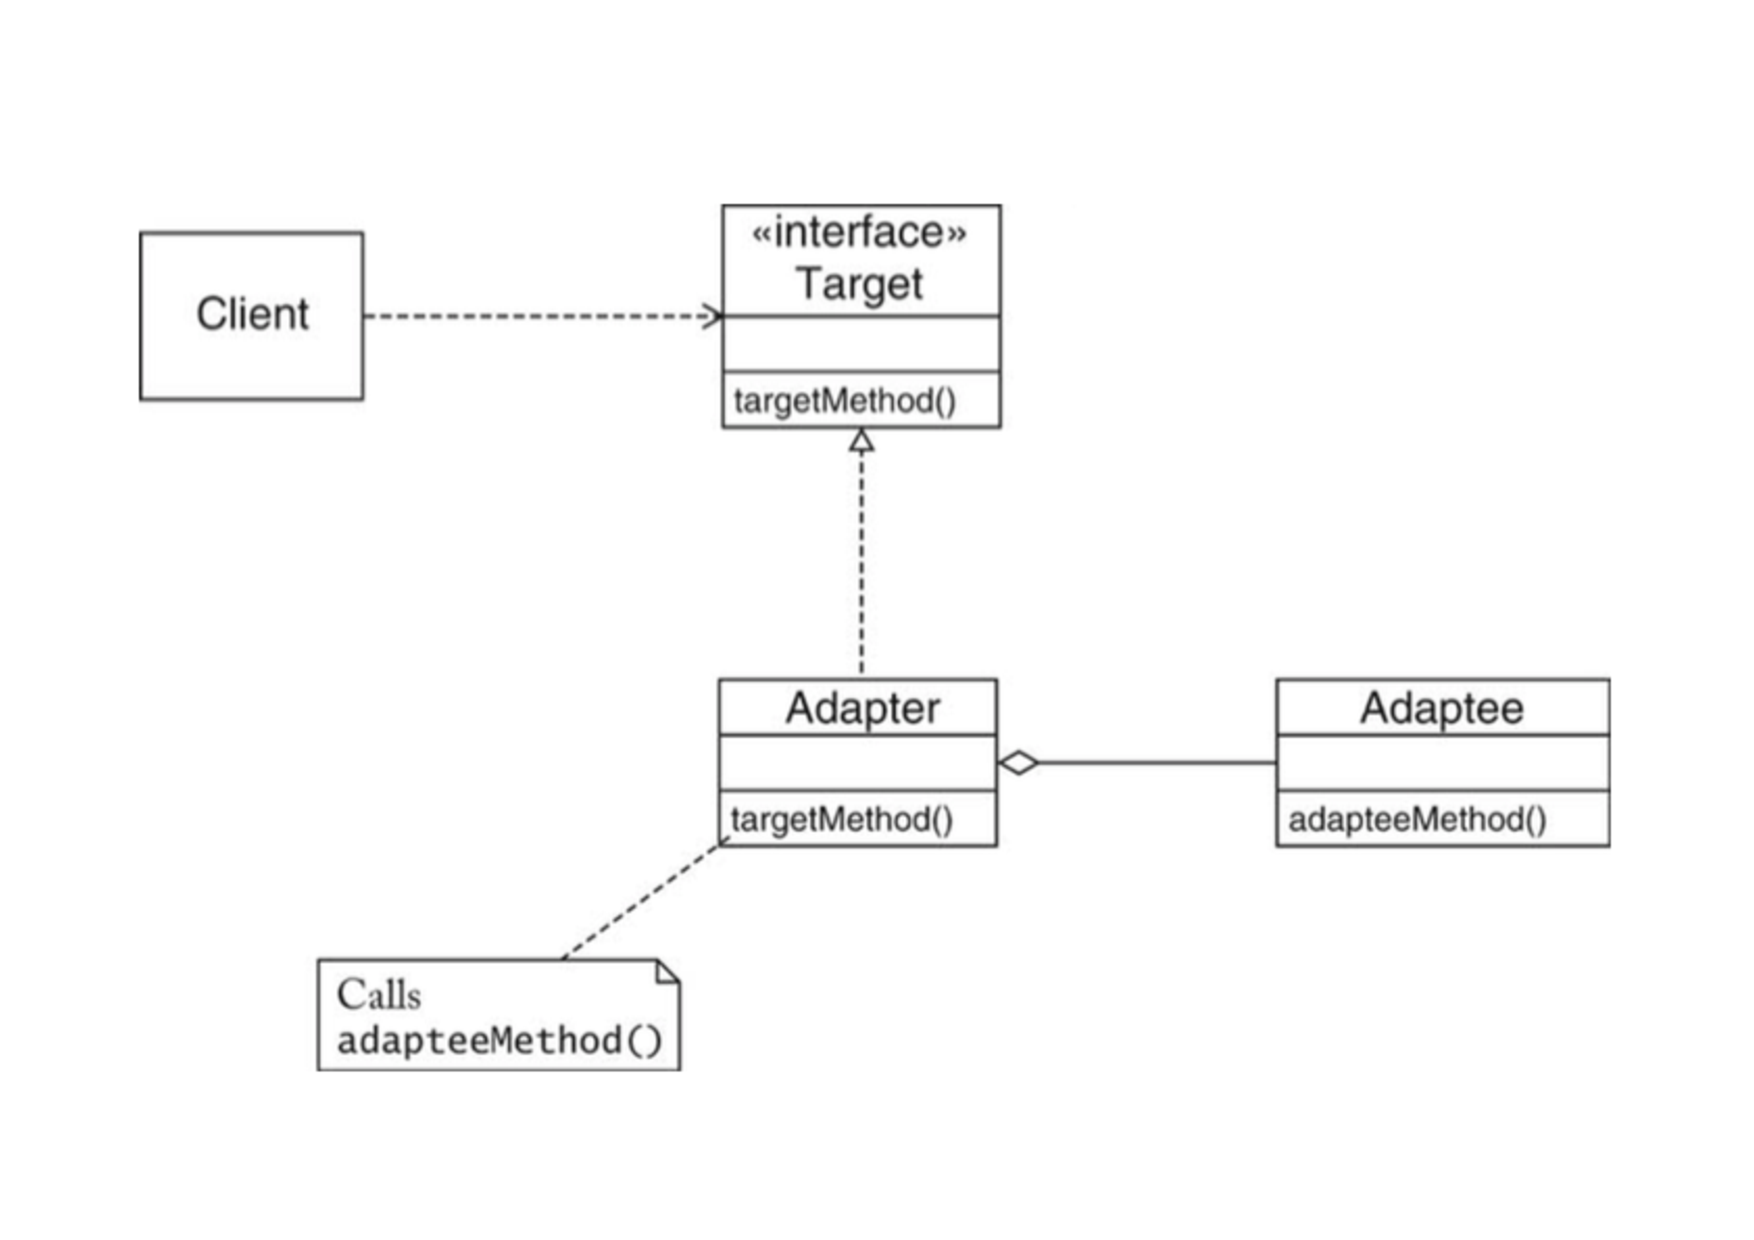
\includegraphics[width=0.7\textwidth]{Img/Adapter.pdf}
\caption{Class diagram relativo al pattern Adapter}
\label{Fig:FactoryAdapterConcepts}
\end{figure}


\noindent Il class diagram riferito al pattern adapter \`e descritto in Figura~\ref{Fig:FactoryAdapterConcepts}. I componenti principali sono:
\begin{itemize}
\item Target (\texttt{Shape}): definisce l'interfaccia (o la classe astratta) che il client desidera utilizzare
\item Client (\texttt{DrawingEditor}): contiene l'oggetto che utilizza la specifica interfaccia
\item Adaptee (\texttt{Cerchio, Rettangolo}): contiene la classe (o l'interfaccia) i cui metodi deveono essere adattati
\item Adapter (\texttt{CerchioShape}): adatta l'interfaccia dell'oggetto da adattare Adaptee all'interfaccia richiesta \texttt{Target}
\end{itemize}

\subsubsection{Proxy}
\begin{framed}
\emph{Fornisce un surrogato o un placeholder di un altro oggetto permettendo di controllarne l'accesso}
\end{framed}
Potrebbero sorgere delle motivazioni a fronte delle quali \`e necessario controllare l'accesso a uno specifico oggetto del nostro sistema. In genere le ragioni sono da ricercare in due categorie:
\begin{itemize}
\item \emph{sicurezza}: non vogliamo consentire di eseguire determinate operazioni su un oggetto.
\item \emph{efficienza}: per esempio vogliamo introdurre una chache che migliora l'efficienza nella risposta agli utenti.
\end{itemize}

In merito all'efficienza possiamo immaginare di non voler pagari i costi della creazione e inizializzazione di un oggetto finch\`e l'oggetto non \`e effettivamente creato. Per esempio, immaginiamo di avere un documento contenente degli elementi tra cui delle immagini. Vorremmo evitare di creare tutte le immagini all'inizio, quando il documento \`e aperto. Per questo, al posto di passare alla classe Document (client) una istanza di un oggetto Immagine (RealSubject) possiamo passare un istanza di ProxyImage (Proxy). Un oggetto di tipo ProxyImage incapsula l'oggetto immagine ma carica l'immagine dal file solo quando \`e necessaria, per esempio solo quando deve essere visualizzata (raggiunta nello scrolling).


Relativamente alla sicurezza una delle ragioni che potrebbero indurci a utilizzare un proxy \`e quella di rendere una collection non modificabile. Questo \`e per esempio il caso delle \emph{unmodifiable Collections}. In questo caso lo scopo \`e quello di non consentire a una collezione di essere modificabile. Per questo, quando vengono chiamati i metodi che modificano la collezione, per esempio  \texttt{add}, viene lanciata l'eccezione \texttt{UnsupportedOperationException}.


\begin{figure}
\centering
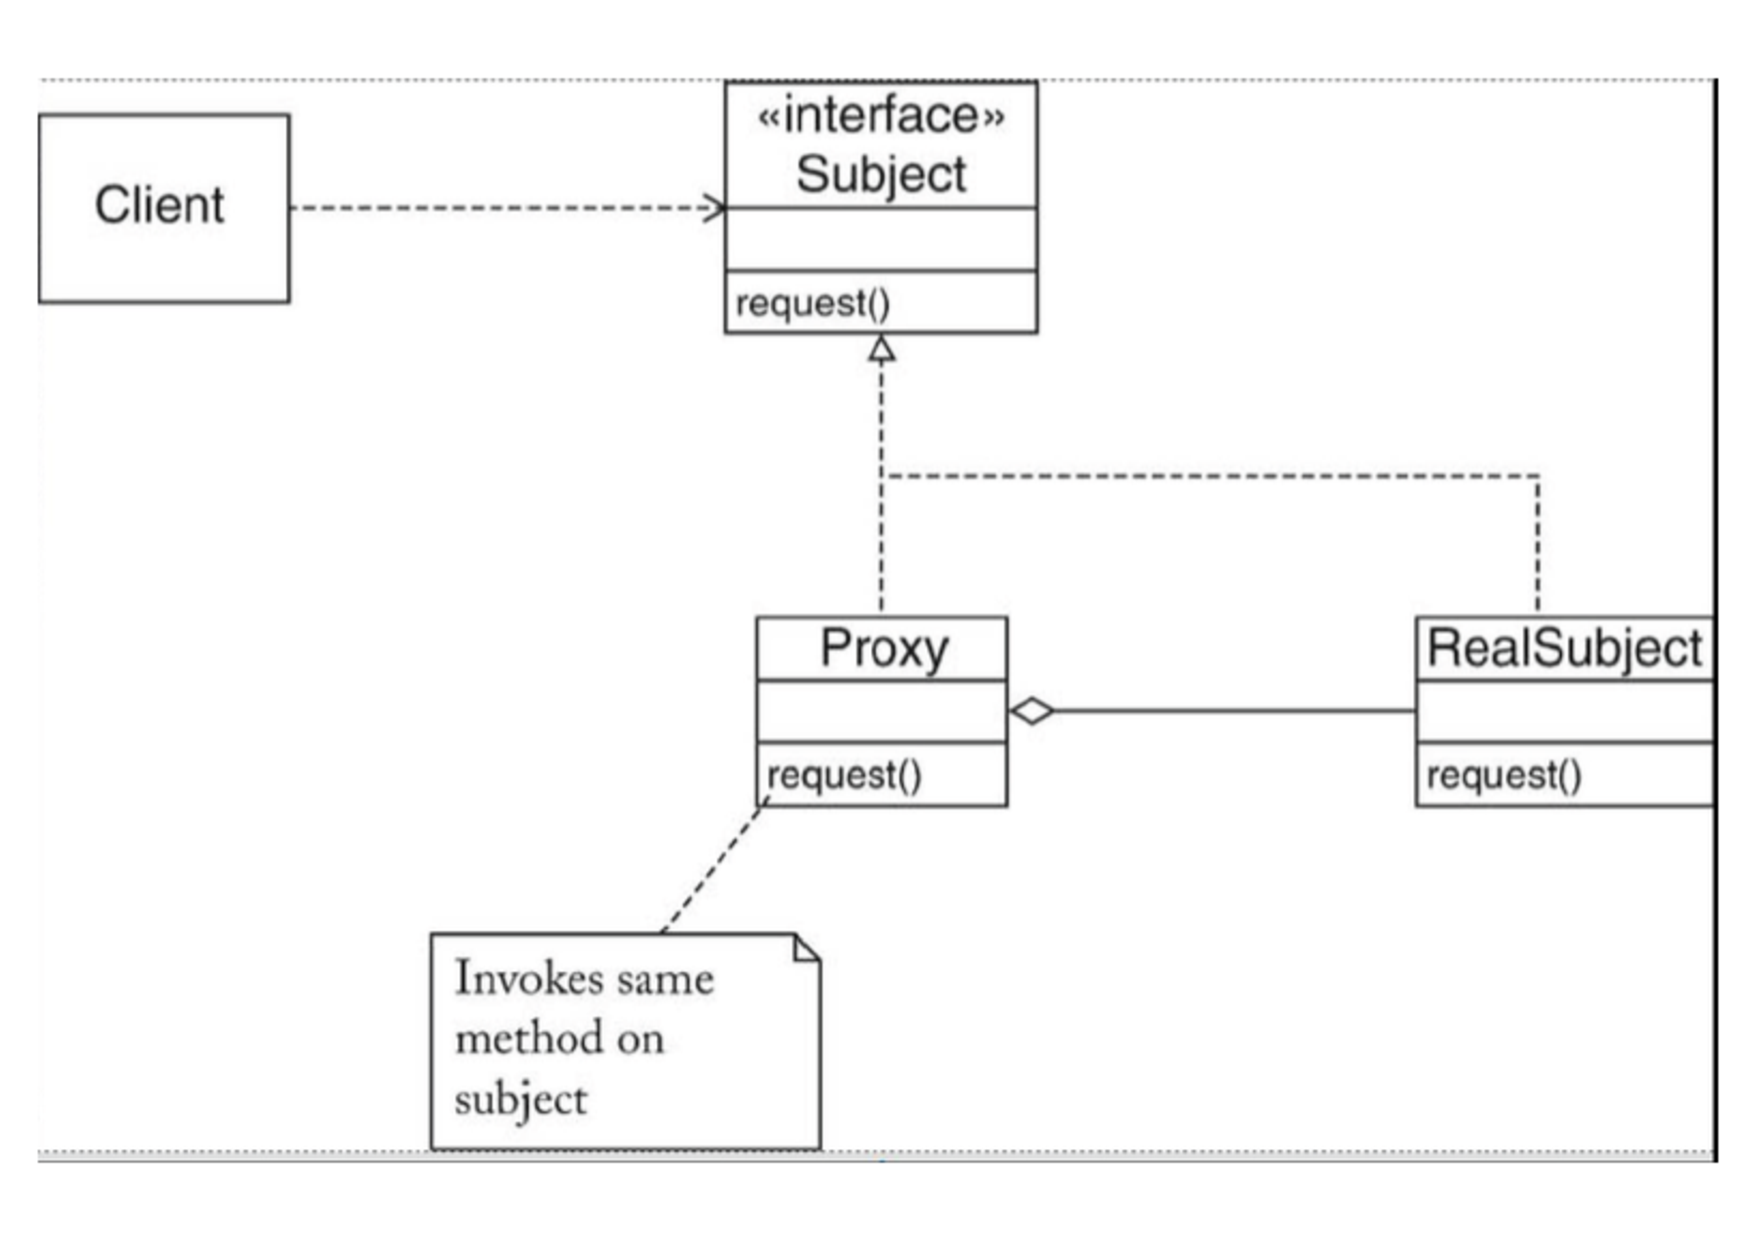
\includegraphics[width=0.7\textwidth]{Img/Proxy.pdf}
\caption{Class diagram relativo al pattern Proxy}
\label{Fig:ProxyAdapterConcepts}
\end{figure}

\noindent Il class diagram riferito al pattern adapter \`e descritto in Figura~\ref{Fig:ProxyAdapterConcepts}. I componenti principali sono:
\begin{itemize}
\item Subject (\texttt{Elemento}): definisce l'interfaccia (o la classe astratta) che il client desidera utilizzare
\item Client (\texttt{Documento}): contiene l'oggetto che utilizza la specifica interfaccia
\item Proxy (\texttt{ImmagineProxy}): contiene la classe dell'elemento proxy
\item RealSubject (\texttt{Immagine}): contiene l'immagine reale che l'elemento proxy rappresenta.
\end{itemize}

Nota che:
\begin{itemize}
\item il proxy fornisce un interfaccia \emph{identica} a quella dell'oggetto che deve essere sostituito all'oggetto reale. 
\item Il proxy controlla l'accesso all'oggetto reale
\item il proxy pu\'o modificare i vari metodi (per esempio nel caso dell'esempio relativo alla sicurezza)
\end{itemize}

Differenze tra proxy e altri patterns:
\begin{itemize}
\item un \emph{adapter} fornisce un interfaccia \emph{diversa} rispetto a quella dell'elemento che ``adatta"
\item un \texttt{decorator} aggiunge responsabilit\`a a un oggetto mentre un proxy ha il ``solo" compito di regolarne l'accesso.
\end{itemize}

\subsubsection{Decorator}
\begin{framed}
\emph{Aggiunge responsabilit\`a addizionali a un oggetto dinamicamente. Fornisce un ottima e flessibile alternativa al \emph{subclassing}}. Aggiungere responsabilit\`a dinamicamente a oggetti individuali.
\end{framed}

A volte lo sviluppatore vorrebbe \emph{aggiungere responsabilit\`a dinamicamente a oggetti individuali}. Immaginiamo per esempio di considerare un tool grafico. Vorremmo controllare a \emph{run-time} quando aggiungere o rimuovere un bordo. Possiamo pensare a varie alternative: aggiungere un booleano che ci permette di visualizzare o meno un bordo, effettuare sub-classing e dichiarare varie classi diverse a seconda che il bordo sia presente o meno. In entrambi i casi le soluzioni posposte sono poco flessibili. Nel primo caso il nostro oggetto a tutti gli effetti ha un bordo, il booleano ci dice solo se il bordo viene visualizzato o meno. Nel secondo caso la scelta relativa al fatto che una classe abbia o meno un bordo viene fatta staticamente.


Un approccio pi\`u flessibile consiste nell'utilizzo di un \emph{decorator}. L'idea \`e molto semplice: per aggiungere un bordo \`e sufficiente encapsulare un oggetto in un altro oggetto che aggiunge un bordo: un \emph{decorator} appunto. Il decorator ha la \emph{stessa interfaccia} del componente che decora per cui la sua presenza \`e trasparente a un client. Il decorator chiama i metodi dell'oggetto che incapsula, ma li pu\`o appunto decorare eseguendo azioni addizionali. Il fatto che il decoratore sia trasparente permette di includere il decoratore in un altro decoratore ricorsivamente (una specie di matrioska di decoratori) in cui ogni decoratore decora le funzionalit\`a di quello che contiene.

Consideriamo un visualizzatore di documenti di testo. Il documento potrebbe essere decorato con dei bordi, poi con delle scrollbar encapsulato in un altro documento che a sua volta contiene scrollbar e bordi.




\begin{figure}[h]
\centering
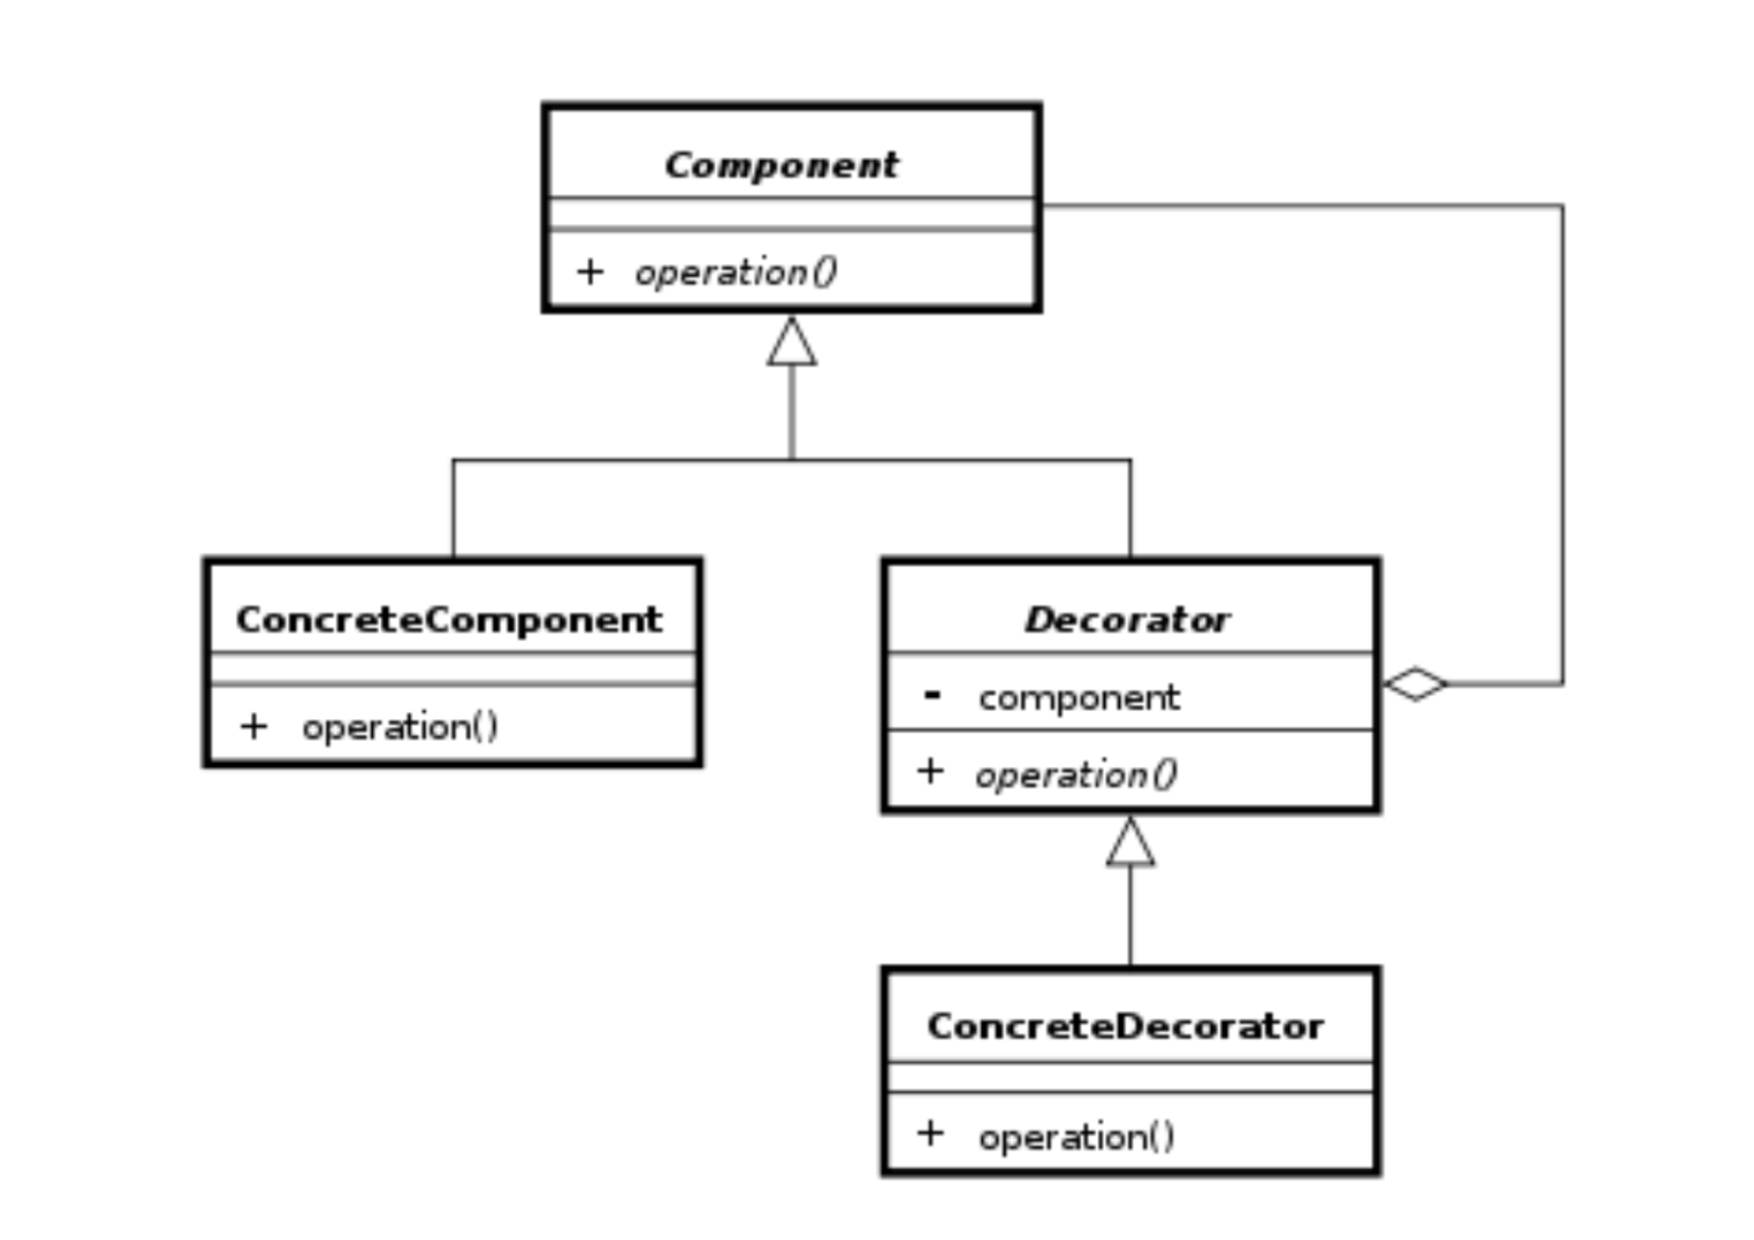
\includegraphics[width=0.7\textwidth]{Img/Decorator.pdf}
\caption{Class diagram relativo al pattern Decorator}
\label{Fig:DecoratorConcepts}
\end{figure}

\`E consigliabile utilizzare il pattern decorator quando:
\begin{itemize}
\item si desidera aggiungere responsabilit\`a a oggetti individuali in maniera dinamica e trasparente
\item quando l'espansione mediante sottoclassi \`e impraticabile (non \`e possibile considerare ogni possibile combinazione).
\end{itemize}

\noindent Il class diagram riferito al pattern adapter Decorator \`e descritto in Figura~\ref{Fig:DecoratorConcepts}. I componenti principali sono:
\begin{itemize}
\item Component (\texttt{ElementoDisegnabile}): definisce l'interfaccia (o la classe astratta) che l'elemento desiderato deve implementare desidera utilizzare
\item ConcreteComponent (\texttt{Documento}): contiene l'oggetto al quale delle responsabilit\`a vanno aggiunte dinamicamente
\item Decorator (\texttt{Decorator}): mantiene il \emph{reference} all'interfaccia del componente contenuto nel decoratore
\item ConcreteDecorator (\texttt{BorderElement, ScrollElement}): contiene il decoratore concreto che pu\`o essere utilizzato per decorere il componente concreto o la ``sua versione gi\`a decorata".
\end{itemize}


Differenze tra decorator e altri patterns:
\begin{itemize}
\item uno \emph{adapter} cambia l'interfaccia un decorator no
\item uno \emph{strategy} \`e molto simile a un decorator. Il decorator cambia la buccia, il contorno, decora un elemento, uno strategy cambia il nocciolo, l'involucro del componente
\end{itemize}

Un approccio simile \`e usato nelle classi per l'input/output di Java.


\subsection{Pattern comportamentali}

\subsubsection{Strategy}
\begin{framed}
\emph{Viene utilizzato quando abbiamo varie strategie (algoritmi) per raggiungere un determinato scopo}
\end{framed}

Supponiamo per esempio di voler realizzare un sistema che splitta un testo in vari paragrafi. A seconda di come viene creato il testo, per esempio la codifica utilizzata dal sistema operativo, o lo specifico editor utilizzato per creare il testo potremmo avere diverse codifiche dello stesso. Quindi il nostro sistema deve utilizzare algoritmi (strategie) differenti a seconda del testo analizzato.

\`E consigliabile utilizzare il pattern strategy quando:
\begin{itemize}
\item ci sono delle classi che si differenziano \emph{solo} per il loro comportamento. Il pattern strategy permette di dichiarare un classe con uno o pi\`u di questi comportamenti
\item servono varie strategie, per esempio strategie ottimizzate rispetto a tempo e/o spazio.
\end{itemize}

\begin{figure}[h]
\centering
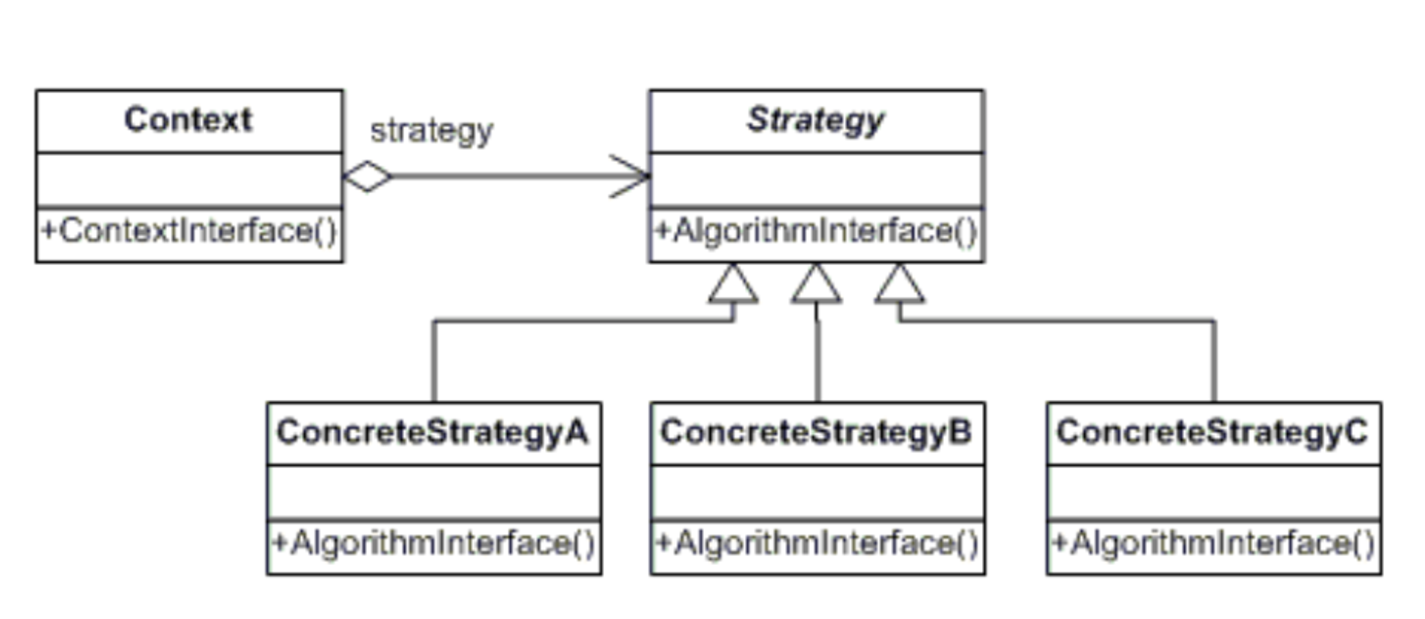
\includegraphics[width=0.7\textwidth]{Img/Strategy.pdf}
\caption{Class diagram relativo al pattern Strategy}
\label{Fig:StrategyConcepts}
\end{figure}

Il class diagram riferito al pattern adapter Strategy \`e descritto in Figura~\ref{Fig:StrategyConcepts}. I componenti principali sono:
\begin{itemize}
\item Context: viene configurato con la strategia da utilizzare. \emph{Mantiene un riferimento alla strategia da utilizzare}
\item Strategy: dichiara un interfaccia comune a tutti gli algoritmi
\item ConcreteStrategy: implementa un algoritmo con la specifica strategia
\end{itemize}

Lo strategy pattern offre i seguenti benefici:
\begin{itemize}
\item fornendo un interfaccia unica \`e possibile creare in modo semplice famiglie di algoritmi mediante opportune gerarchie
\item \`e possibile creare sottoclassi di context che forzano l'uso di un algoritmo preciso. In tal caso valgono gli stessi ragionamenti fatti nell'esercitazione di UML per la relazione tra Benefit e funzionalit\`a
\item il pattern strategy offre un ottimo modo per rimuovere costrutti \emph{if-else} dal codice 
\end{itemize}

\subsubsection{Observer}
\begin{framed}
\emph{Definisce una dipendenza tra oggetti nella quale quando un oggetto \emph{cambia stato} tutti gli oggetti dipendenti da qull'oggetto vengono notificati}
\end{framed}

\`E anche conosciuto come \textbf{Publish-Subscribe}.

Un problema ben noto quando si divide un sistema in varie parti/vari componenti \`e mantenere la consistenza tra gli oggetti relazionati. Tuttavia, si vuole evitare di ``accoppiare in maniera forte i vari" componenti visto che queste scelte riducono la riusabilit\`a. Si vuole un pattern generico che consenta di riutilizzare le varie parti del sistema.

Supponiamo per esempio di voler sviluppare un foglio di calcolo. \`E interessante avere da una parte i dati, dall'altra parte vari grafici che ci consento di visualizzare questi dati. Quando i dati cambiano si vorrebbe che i corrispettivi grafici vengano aggiornati. Tuttavia si vuole garantire la riusabilit\`a. Uno diagramma a barre potrebbe essere utilizzato per visualizzare anche altri tipi di informazioni.

\begin{figure}[h]
\centering
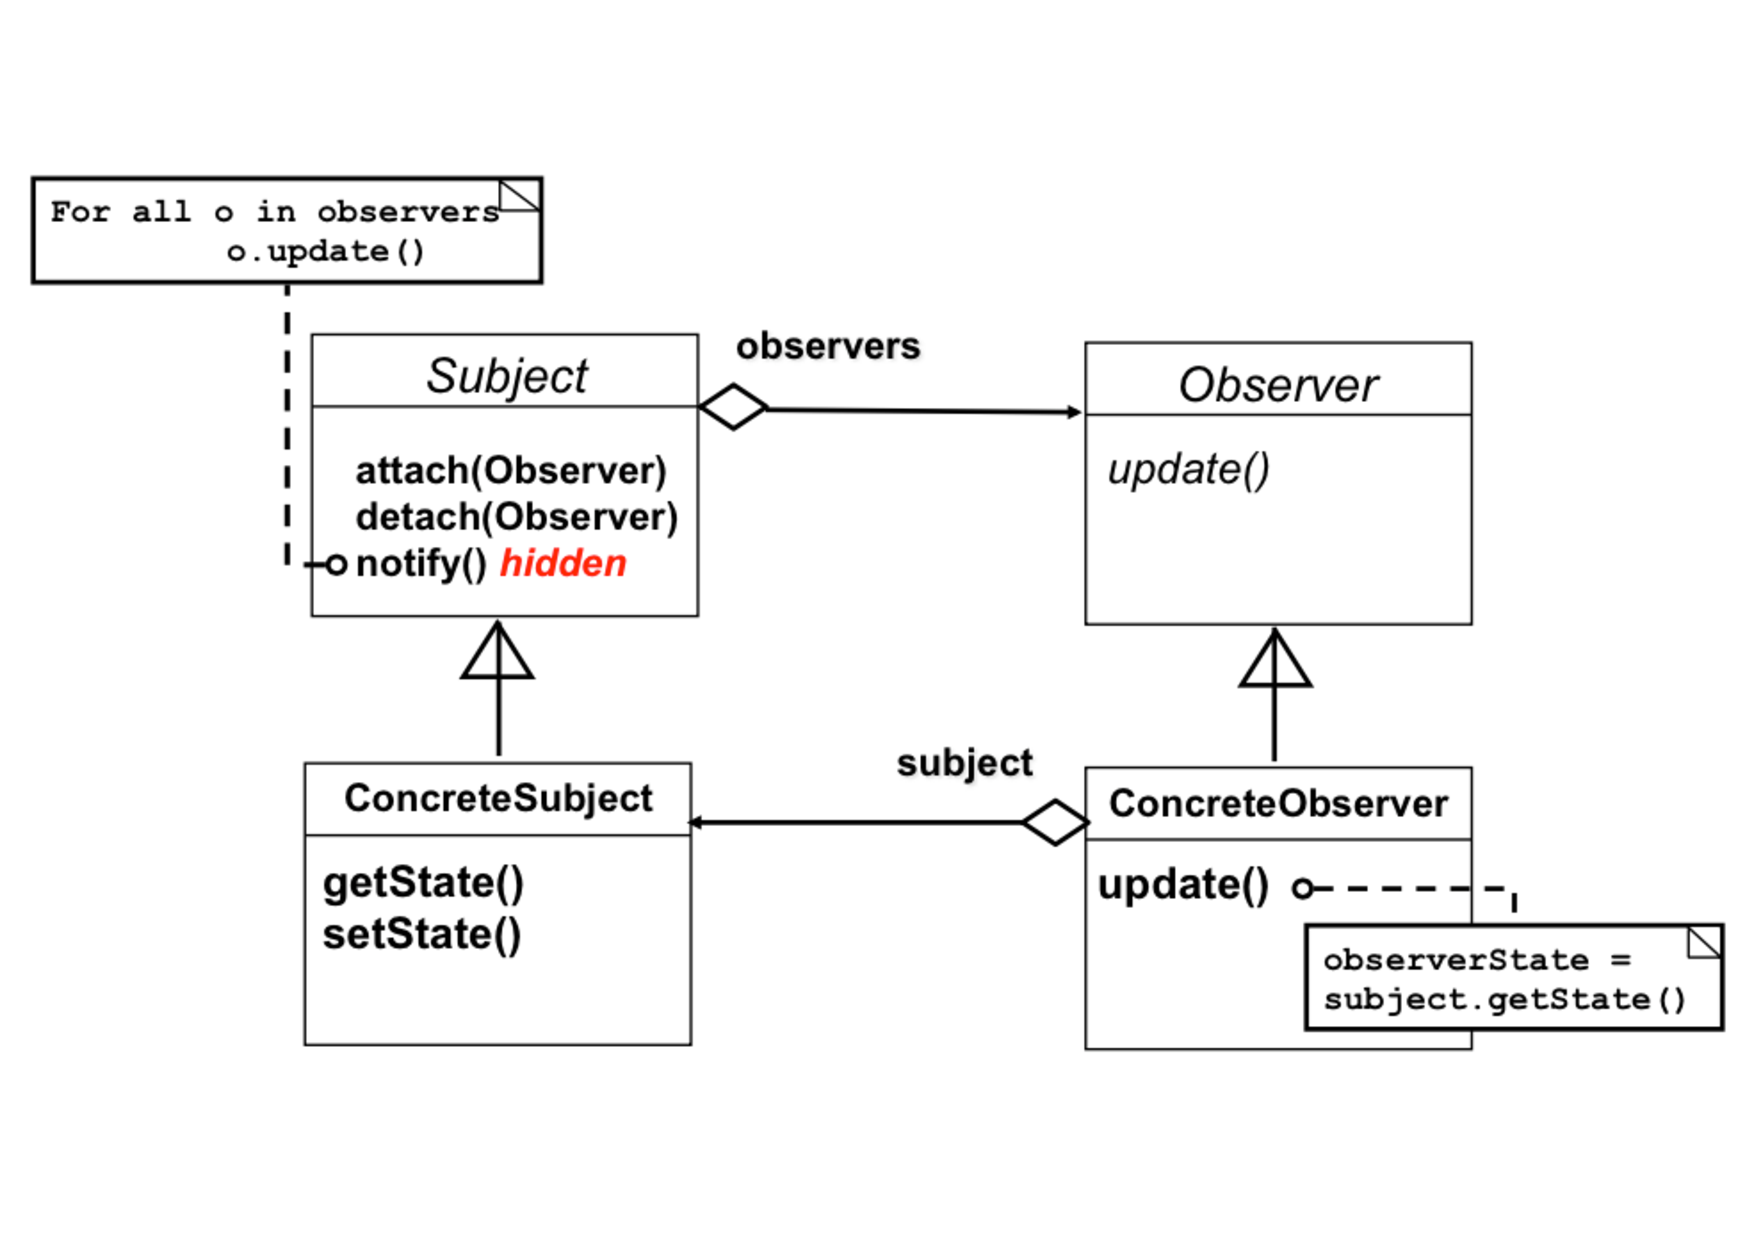
\includegraphics[width=0.7\textwidth]{Img/Observer.pdf}
\caption{Class diagram relativo al pattern Observer}
\label{Fig:ObserverConcepts}
\end{figure}

Il pattern \emph{observer} fa al caso nostro. Gli elementi chiave in questo contesto sono un osservatore e il soggetto che viene osservato. Un soggetto osservato pu\`o avere un numero qualsiasi di osservatori.  Tutti gli osservatori sono notificati quando un soggetto cambia il proprio stato. \emph{In risposta a questa notifica gli osservatori eseguiranno delle query sullo stato dell'osservato per sincronizzarsi con il nuovo stato.}

\`E consigliabile utilizzare il pattern Observer quando:
\begin{itemize}
\item quando l'applicazione ha due parti ben distinte una dipendente dall'altra, che si desidera riutilizzare in maniera indipendente
\item quando un cambiamento in uno dei due oggetti richiede di cambiare altri oggetti e non si conosce a priori quali saranno gli oggetti da cambiare
\item quando un oggetto deve \emph{notificare} altri oggetti senza poter fare assunzioni su chi saranno questi altri oggetti
\end{itemize}

Il class diagram riferito al pattern adapter Observer \`e descritto in Figura~\ref{Fig:ObserverConcepts}. I componenti principali sono:
\begin{itemize}
\item Subject: classe che specifica come gestire gli osservatori. Contiene il riferimento degli osservatori e l'implementazione del metodo notify e i metodi per attaccare e rimuovere degli osservatori
\item Observer: definisce e aggiorna l'interfaccia degli oggetti che devono essere notificati al cambiare di un oggetto
\item ConcreteSubject: \`e l'elemento che deve essere effettivamente monitorato dall'observer. Contiene lo stato dell'elemento. Ricorda quando lo stato viene cambiato lo sviluppatore deve invocare il metodo \emph{notify}
\item ConcreteObserver: mantiene un rierimento al concreteSubject monitorato. Implementa l'interfaccia \texttt{Observer}.
\end{itemize}

Il pattern observer offre i seguenti benefici:
\begin{itemize}
\item fornisce una relazione astratta tra il soggetto e il suo osservatore. Il soggetto "Astratto" (Subject) conosce la lista dei suoi osservatori, ma non conosce il tipo specifico di questi osservatori, conosce solamente che implementano \texttt{Observer}. Questo consente di relazionare elementi che appartengono a diversi livelli di astrazione (per esempio un elemento di basso livello potrebbe comunicare il suo stato a un elemento di alto livello lasciando la loro struttura intatta). Nota la lista degli osservatori potrebbe ``essere mascherata" a concrete subject. Per esempio potrebbe essere dichiarate \texttt{private} all'interno di \texttt{Subject} senza che \texttt{Subject} esponga getter e setted relativi agli osservatori, ma solo esponendo il metodo \texttt{notifyAll()}. In questo caso il concreteSubject, pu\`o solo invocare il metodo \texttt{notifyAll()} senza che possa conoscere la lista dei suoi osservatori.
\item la notifica che un elemento \`e cambiato viene mandata in broadcast. Al soggetto non interessa quanti sono gli oggetti interessati ne quali sono. L'unico suo interesse \`e nel mandare la notifica
\item ATTENZIONE! se nella gestione dell'update all'interno dell'obsever viene cambiato lo stato del soggetto concreto potrebbero esserci modifiche a cascata e potenzialemente si potrebbe entrare in un loop. Per esempio se uno degli osservatori mette un attributo \texttt{x} a 1 un altro osservatore mette l'attributo \texttt{x} a zero all'interno della gestione di un update. 
\end{itemize}

Note implementative e possibili variazioni:
\begin{itemize}
\item un osservatore potrebbe osservare pi\`u soggetti. In tal caso \`e necessario estendere l'interfaccia update per consentire all'osservatore di conoscere l'oggetto che ha chiamato il metodo update
\item bisogna prestare attenzione a quando si elimina un osservatore o un osservato ad eliminare il corrispettivo reverence dall'osservato e dagli osservatori, rispettivamente.
\item \`e possibile specificare all'interno della notify la parte dell'elemento cambiato (Aspect)
\item \`e anche possibile interporre tra osservatore e osservato un \texttt{ChangeManager} in caso che gli update siano complessi o si debba specificare particolari strategie di update
\end{itemize}


\subsubsection{Iterator}
\begin{framed}
\emph{Fornisce un metodo che consente di accedere agli elementi di una oggetto aggregato (che contiene altri elementi) in maniera sequenziale senza esporre la rappresentazione dell'oggetto aggregato}
\end{framed}
Per i dettagli teorici il lettore \`e rimandato alla corrispondente lezione.
\clearpage
\section{Esercizi}




\subsection{Adapter/Wrapper}
\Esercizio{\begin{itemize}
\item Vogliamo sviluppare una applicazione che permetta l'utilizzo di diverse tecnologie di comunicazione, evitando il pi\`u possibile duplicazioni di codice
\item come possiamo strutturare la nostra applicazione?
\item supponiamo per esempio di avere la nostra logica che ci consente di eseguire un set di operazioni \texttt{action(A)},  \texttt{action(B)} and  \texttt{action(C)} come possiamo supportare un client che utilizza dei comandi specificati per mezzo di Stringhe o vari tipi di comunicazione?  
\end{itemize}
}

In genere si
\begin{itemize}
\item scrive la logica applicativa indipendentemente dal protocollo utilizzato. 
\item Implementano le classi per permettere la comunicazione
\item adatta il comportamento della classe a quello richiesto dal protocollo
\end{itemize} 

La classe \texttt{SocketInterface} specifica il ``protocollo" (interfaccia) esposta dal server al client. La logica applicativa \texttt{ApplicationLogic} viene sviluppata in modo indipendente al canale di comunicazione utilizzato. Al fine di adattare la logica applicativa alla particolare interfaccia utilizzata \`e bene utilizzare degli opportuni adapter. Nel caso considerato \texttt{SocketAdapter} viene utilizzato per adattare la logica applicativa all'utilizzo di un interfaccia socket.

Nota: l'esempio e l'implementazione sono forniti con il \emph{solo} fine di illustrare il pattern adapter. Non si pongono come obiettivo quello di implementare una comunicazione per mezzo di socket funzionante che sar\`a trattata in seguito.



\begin{figure}[h]
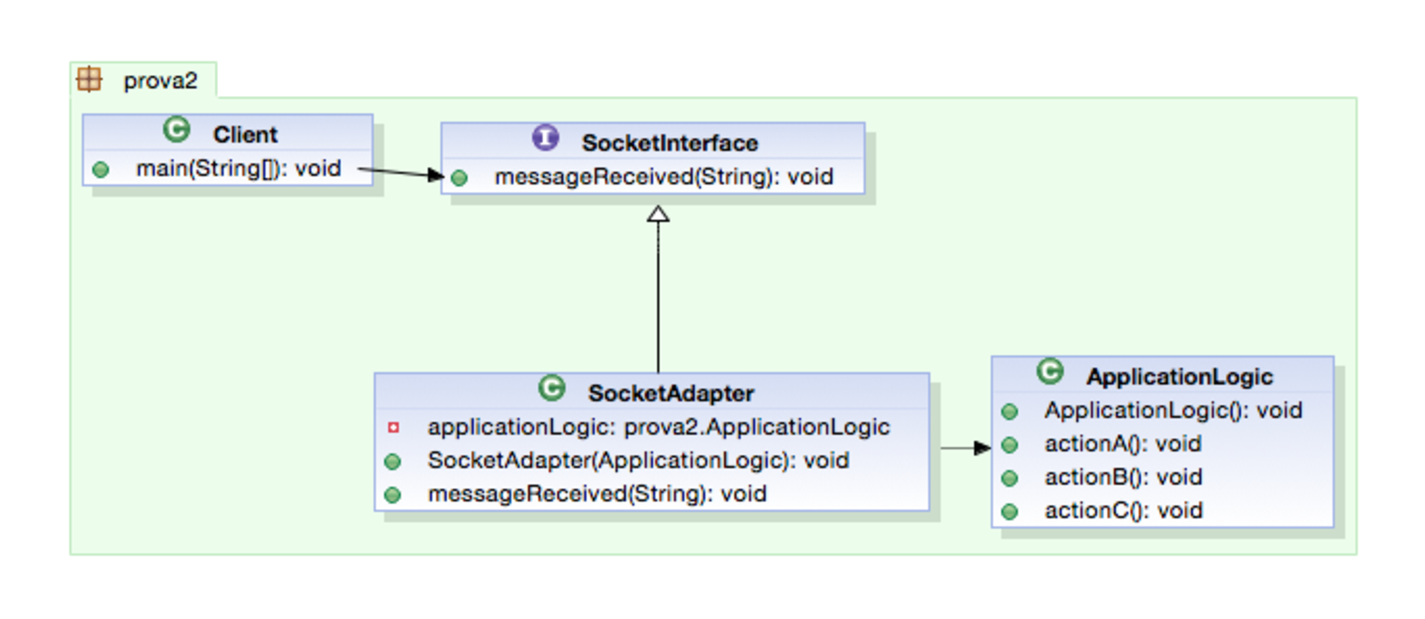
\includegraphics[width=1\textwidth]{Img/AdapterEsercizio1.pdf}
\caption{Class Diagram relativo alla soluzione dell'esercizio 1. Il diagramma \`e stato generato partendo dal codice utilizzando il tool descritto in laboratorio. Per questo il diagramma \`e lievemente divers da quello presentato in Figura~\ref{Fig:FactoryAdapterConcepts}}
\label{Fig:AdapterEsercizio1}
\end{figure}

\begin{lstlisting}[language=Java]
public class ApplicationLogic {
    public void actionA(){
    	System.out.println("Logica: Eseguo il metodo A");
    }
    public void actionB(){
    	System.out.println("Logica: Eseguo il metodo B");
    }
    public void actionC(){
    	System.out.println("Logica: Eseguo  il metodo C");
    }
 }
\end{lstlisting}

\begin{lstlisting}[language=Java]
public interface SocketInterface {
	public void messageReceived(String message);
}
\end{lstlisting}

\begin{lstlisting}[language=Java]
public class SocketAdapter implements SocketInterface{
	
	// contiene la logica vera e propria
	private final ApplicationLogic applicationLogic;
	
	public SocketAdapter(ApplicationLogic applicationLogic){
		this.applicationLogic=applicationLogic;
	}
	
	
	public void messageReceived(String message){
		// gestisce il protocollo
		if(message.equals("A")){
			applicationLogic.actionA();
		}
		if(message.equals("B")){
			applicationLogic.actionB();
		}
		if(message.equals("C")){
			applicationLogic.actionC();
		}
	}
}
\end{lstlisting}


\begin{lstlisting}[language=Java]
public class Client {

	public static void main(String[] args) {
		ApplicationLogic applicationLogic=new ApplicationLogic();
		SocketInterface socketInterface = new SocketAdapter(applicationLogic);
		socketInterface.messageReceived("A");
	}
}
\end{lstlisting}


\subsection{Proxy}
\Esercizio{Immaginiamo di implementare un social network. Data una specifica persona vorremmo mostrare come ``potenziali amici" gli  amici degli amici degli amici. Come possiamo implementarla in maniera efficace?}

In questo caso \`e naturale immaginarsi che la computazione degli amici degli amici degli amici sia un operazione complessa da un punto di vista computazionale o, in ogni caso un operazione che viene ripetuta pi\`u volte su un determinato utente. Ci viene quindi naturale pensare che \`e possibile implementare la soluzione mediante un \emph{proxy} che svolga la funzione di \emph{cache}. 

Nella soluzione, la nostra applicazione \texttt{ApplicationInterface}, fornisce il metodo \texttt{getPotenzialiAmici}, che data una persona computa i suoi potenziali amici. All'interno della nostra \texttt{ApplicationLogic} implementiamo la logica applicativa includendo l'implementazione del metodo \texttt{getPotenzialiAmici} che ritorna il \texttt{Set} dei possibili amici di una persona. A questo punto decidiamo di implementare la classe \texttt{ApplicationLogicProxy} che implementa la stessa interfaccia di \texttt{ApplicationLogic} ma contiene una mappa, con funzione di cache che data una persona ritorna i suoi potenziali amici senza rieseguire l'algoritmo. Nota, il proxy contiene un riferimento alla corrispondente\texttt{ApplicationLogic} il cui metodo \texttt{getPotenzialiAmici} viene eseguito quando la \texttt{Persona} non \`e in cache.


\begin{figure}[h]
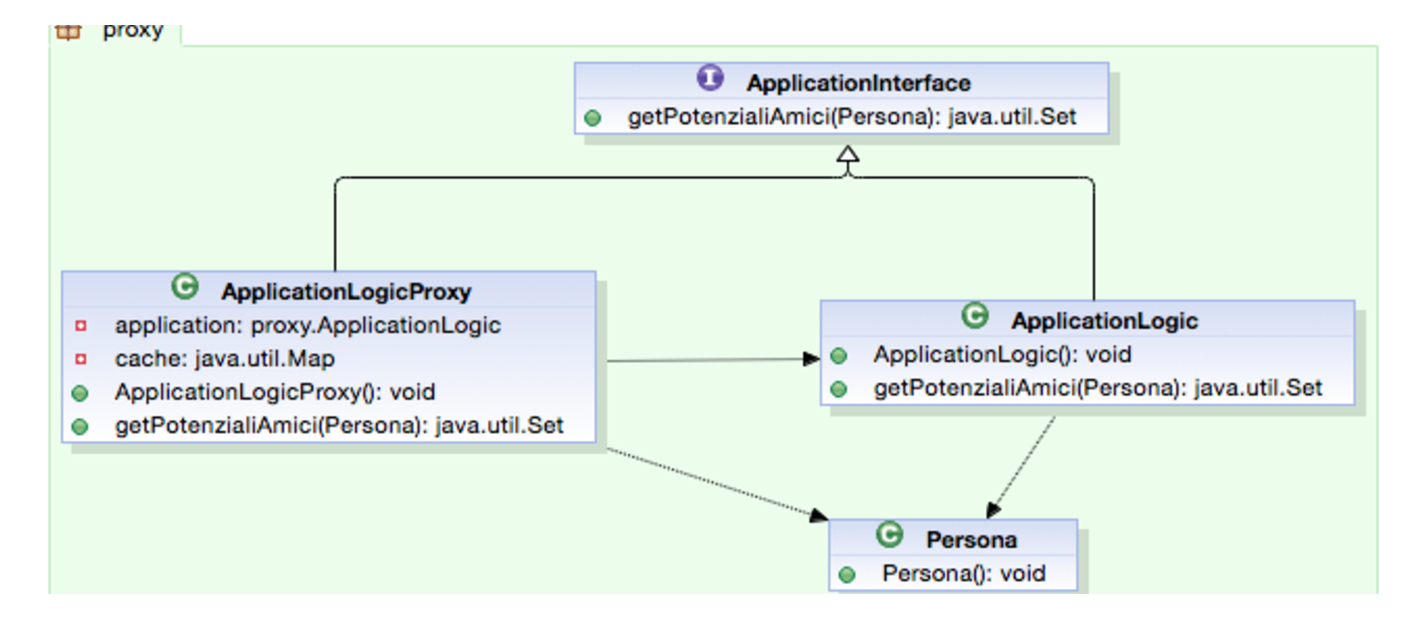
\includegraphics[width=1\textwidth]{Img/ProxyEsercizio1.pdf}
\caption{Class Diagram relativo alla soluzione dell'esercizio 2. Il diagramma \`e stato generato partendo dal codice utilizzando il tool descritto in laboratorio. Per questo il diagramma \`e lievemente divers da quello presentato in Figura~\ref{Fig:ProxyAdapterConcepts}}
\label{Fig:ProxyEsercizio1}
\end{figure}


\begin{lstlisting}[language=Java]
public interface ApplicationInterface {
	
	public Set<Persona> getPotenzialiAmici(Persona p);

}
\end{lstlisting}

\begin{lstlisting}[language=Java]
public class ApplicationLogic implements ApplicationInterface {

	@Override
	public Set<Persona> getPotenzialiAmici(Persona p) {
		// TODO metodo che ritorna i potenziali amici
		
		return null;
	}

}
\end{lstlisting}

\begin{lstlisting}[language=Java]
public class ApplicationLogicProxy implements ApplicationInterface{
	
	private final Map<Persona, Set<Persona>> cache;
	private final ApplicationLogic application;
	
	public ApplicationLogicProxy(){
		this.application=new ApplicationLogic();
		this.cache=new HashMap<Persona, Set<Persona>>();
		
	}
	@Override
	public Set<Persona> getPotenzialiAmici(Persona p) {
		if(!cache.containsKey(p)){
			cache.put(p, application.getPotenzialiAmici(p));
		}
		
		return cache.get(p);
	}
}
\end{lstlisting}

\begin{lstlisting}[language=Java]
public class Persona {
    
}
\end{lstlisting}

\subsection{Decorator}
\Esercizio{Scrivere un applicazione per rappresentare diversi tipi di caff\`e con diversi ingredienti. Per esempio, vorremmo aggiungere del caramello, del whiskey, dello zucchero, a richiesta. Dato un caff\`e vorremmo saperne il costo. Il costo di un caff\`e con un determinato \`e computato in maniera differente a seconda degli ingredienti. Per esempio, l'aggiunta del whiskey al caff\`e potrebbe duplicarne il prezzo, mentre il prezzo del caff\`e zuccherato \`e automentato di 10c.}

La prima idea potrebbe essere quella di fare varie sottoclassi. Ovviamente questa non \`e una buona scelta: ne dovremmo fare troppe. Inoltre non \`e possibile aggiungere nuovi elementi a run time. Inoltre l'aggiunta di un nuovo tipo di elemento comporta modifiche notevoli nel codice.

Il pattern decorator invece fa al caso nostro. Dichiariamo un tipo di caff\`e classico "normale" \texttt{SimpleCoffee} che pu\`o essere decorato con vari elementi zucchero (\texttt{Zucchero}), whiskey (\texttt{Whiskey}) che decorano il caff\`e (aumentandone il costo). 


\begin{figure}[h]
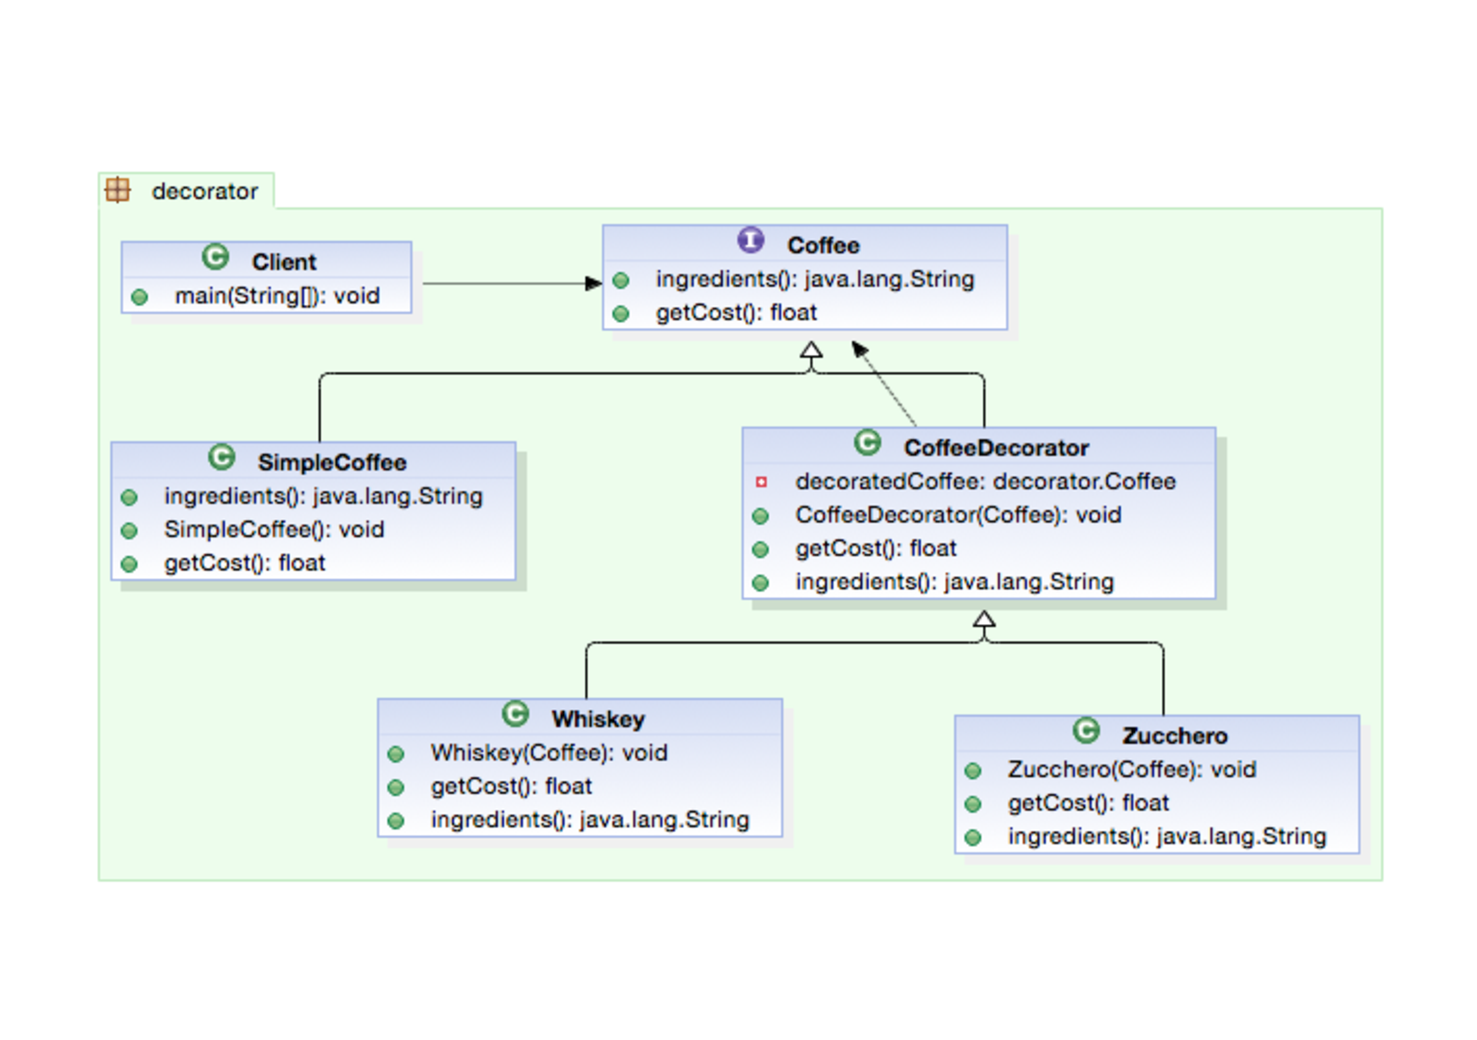
\includegraphics[width=1\textwidth]{Img/DecoratorEsercizio3.pdf}
\caption{Class Diagram relativo alla soluzione dell'esercizio 3. Il diagramma \`e stato generato partendo dal codice utilizzando il tool descritto in laboratorio. Per questo il diagramma \`e lievemente divers da quello presentato in Figura~\ref{Fig:DecoratorConcepts}}
\label{Fig:DecoratorEsercizio3}
\end{figure}

\begin{lstlisting}[language=Java]
public interface Coffee {
	public String ingredients();
	public float getCost();
}
\end{lstlisting}
\begin{lstlisting}[language=Java]
//classe base senza nessuna decorazione
public class SimpleCoffee implements Coffee{

	@Override
	public String ingredients() {
		return "coffee";
	}

	@Override
	public float getCost() {		
		return 1;
	}
}
\end{lstlisting}

\begin{lstlisting}[language=Java]
public abstract class CoffeeDecorator implements Coffee{
	private final Coffee decoratedCoffee;
	public CoffeeDecorator (Coffee decoratedCoffee){
		this.decoratedCoffee = decoratedCoffee;
	}
	@Override
	public String ingredients(){
		return decoratedCoffee.ingredients();
	}
	@Override
	public float getCost(){
		return decoratedCoffee.getCost();
	}
}
\end{lstlisting}

\begin{lstlisting}[language=Java]
public class Zucchero  extends CoffeeDecorator{
	public Zucchero(Coffee decoratedCoffee){
		super(decoratedCoffee);
	}
	
	@Override
	public String ingredients(){
		return "Cocoa " + super.ingredients();
	}
	
	@Override
	public float getCost(){
		return super.getCost() + .1f;
	}
}
\end{lstlisting}

\begin{lstlisting}[language=Java]
public class Whiskey extends CoffeeDecorator {

	public Whiskey(Coffee decoratedCoffee) {
		super(decoratedCoffee);	
	}	
	
	@Override
	public String ingredients(){
		return "Whiskey " + super.ingredients();
	}
	
	@Override
	public float getCost() {
		return super.getCost() * 3;
	}
}
\end{lstlisting}

\begin{lstlisting}[language=Java]
public class Client {
	
	public static void main(String args[]) {
	     Coffee coffe = new SimpleCoffee();
	     Coffee decoratedCoffee = new Whiskey(coffe);
	     System.out.println("coffee: " + decoratedCoffee.ingredients());
	     System.out.println("cost: " + decoratedCoffee.getCost());  
	     
	     decoratedCoffee = new Zucchero(decoratedCoffee);
	     System.out.println("coffee: " + decoratedCoffee.ingredients());
	     System.out.println("cost: " + decoratedCoffee.getCost());  
	}	
}
\end{lstlisting}

\subsection{Strategy}
\Esercizio{Scrivere il codice per rappresentare un robot che pu\`o avere diverse strategie per gestire il suo comportamento. Vogliamo fare si che i comportamenti possano cambiare mentre la nostra applicazione \`e in esecuzione.}


\begin{figure}[h]
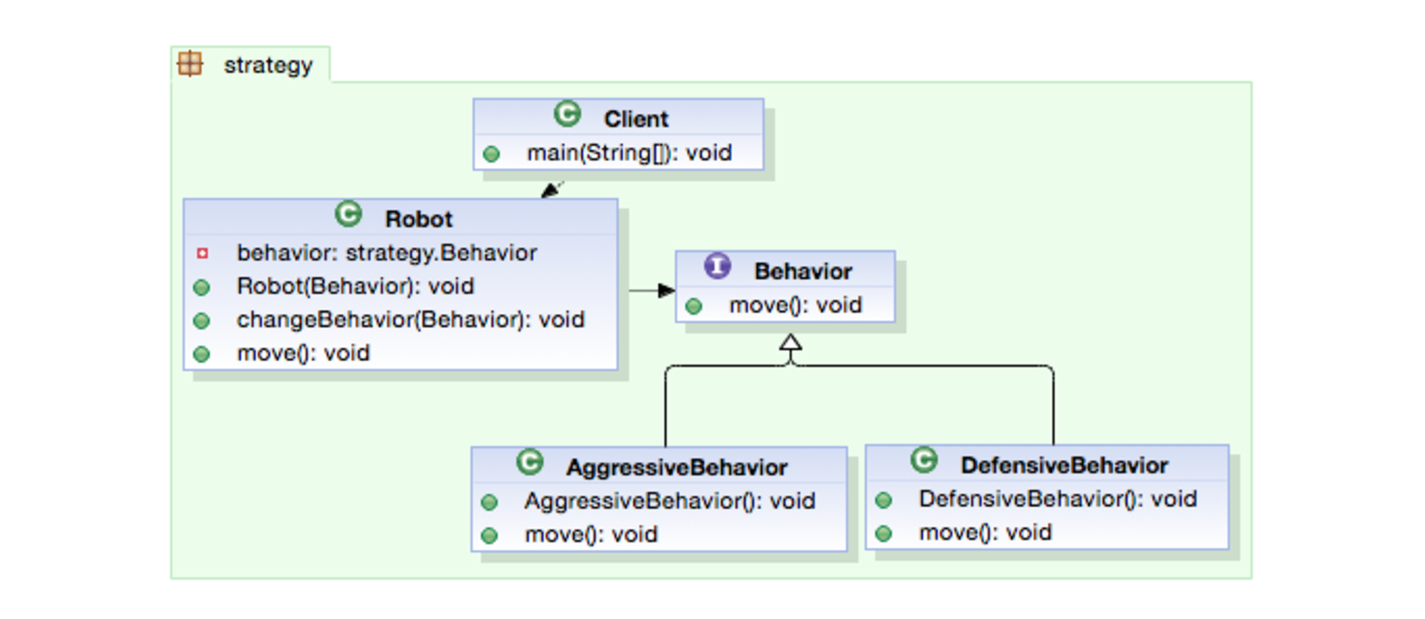
\includegraphics[width=1\textwidth]{Img/StrategyEsercizio4.pdf}
\caption{Class Diagram relativo alla soluzione dell'esercizio 4. Il diagramma \`e stato generato partendo dal codice utilizzando il tool descritto in laboratorio. Per questo il diagramma \`e lievemente divers da quello presentato in Figura~\ref{Fig:StrategyConcepts}}
\label{Fig:strategy}
\end{figure}

\begin{lstlisting}[language=Java]
public class AggressiveBehavior implements Behavior{

	@Override
	public void move() {
		System.out.println("Aggressive move");
		
	}
}
\end{lstlisting}

\begin{lstlisting}[language=Java]
public class DefensiveBehavior implements Behavior{

	@Override
	public void move() {
		System.out.println("Defensive move");
		
	}
}
\end{lstlisting}

\begin{lstlisting}[language=Java]
public interface Behavior {
	public void move();	
}
\end{lstlisting}


\begin{lstlisting}[language=Java]
public class Robot {
	private Behavior behavior;
	
	public Robot(Behavior behavior){
		this.behavior = behavior;		
	}
	
	public void changeBehavior(Behavior behavior){
		this.behavior = behavior;	
	}
	
	public void move(){
		behavior.move();
	}
}
\end{lstlisting}

\begin{lstlisting}[language=Java]
public class Client {
	public static void main(String[] args){
		Robot robot = new Robot(new DefensiveBehavior());
		robot.move();
		robot.changeBehavior(new AggressiveBehavior());
		robot.move();
	}
}
\end{lstlisting}

\subsection{Observer}
\Esercizio{
Progettare un sistema per il monitoraggio del Meteo:
\begin{itemize}
\item si ha a disposizione l'oggetto \texttt{WeatherData} che fornisce temperatura, umidit\`a, pressione
\item implementare tre diversi tipi di display che mostrano condizione attuale, previsioni e statistiche
\item il sistema deve essere espandibile per supportare nuovi display
\end{itemize}
}


\begin{figure}[h]
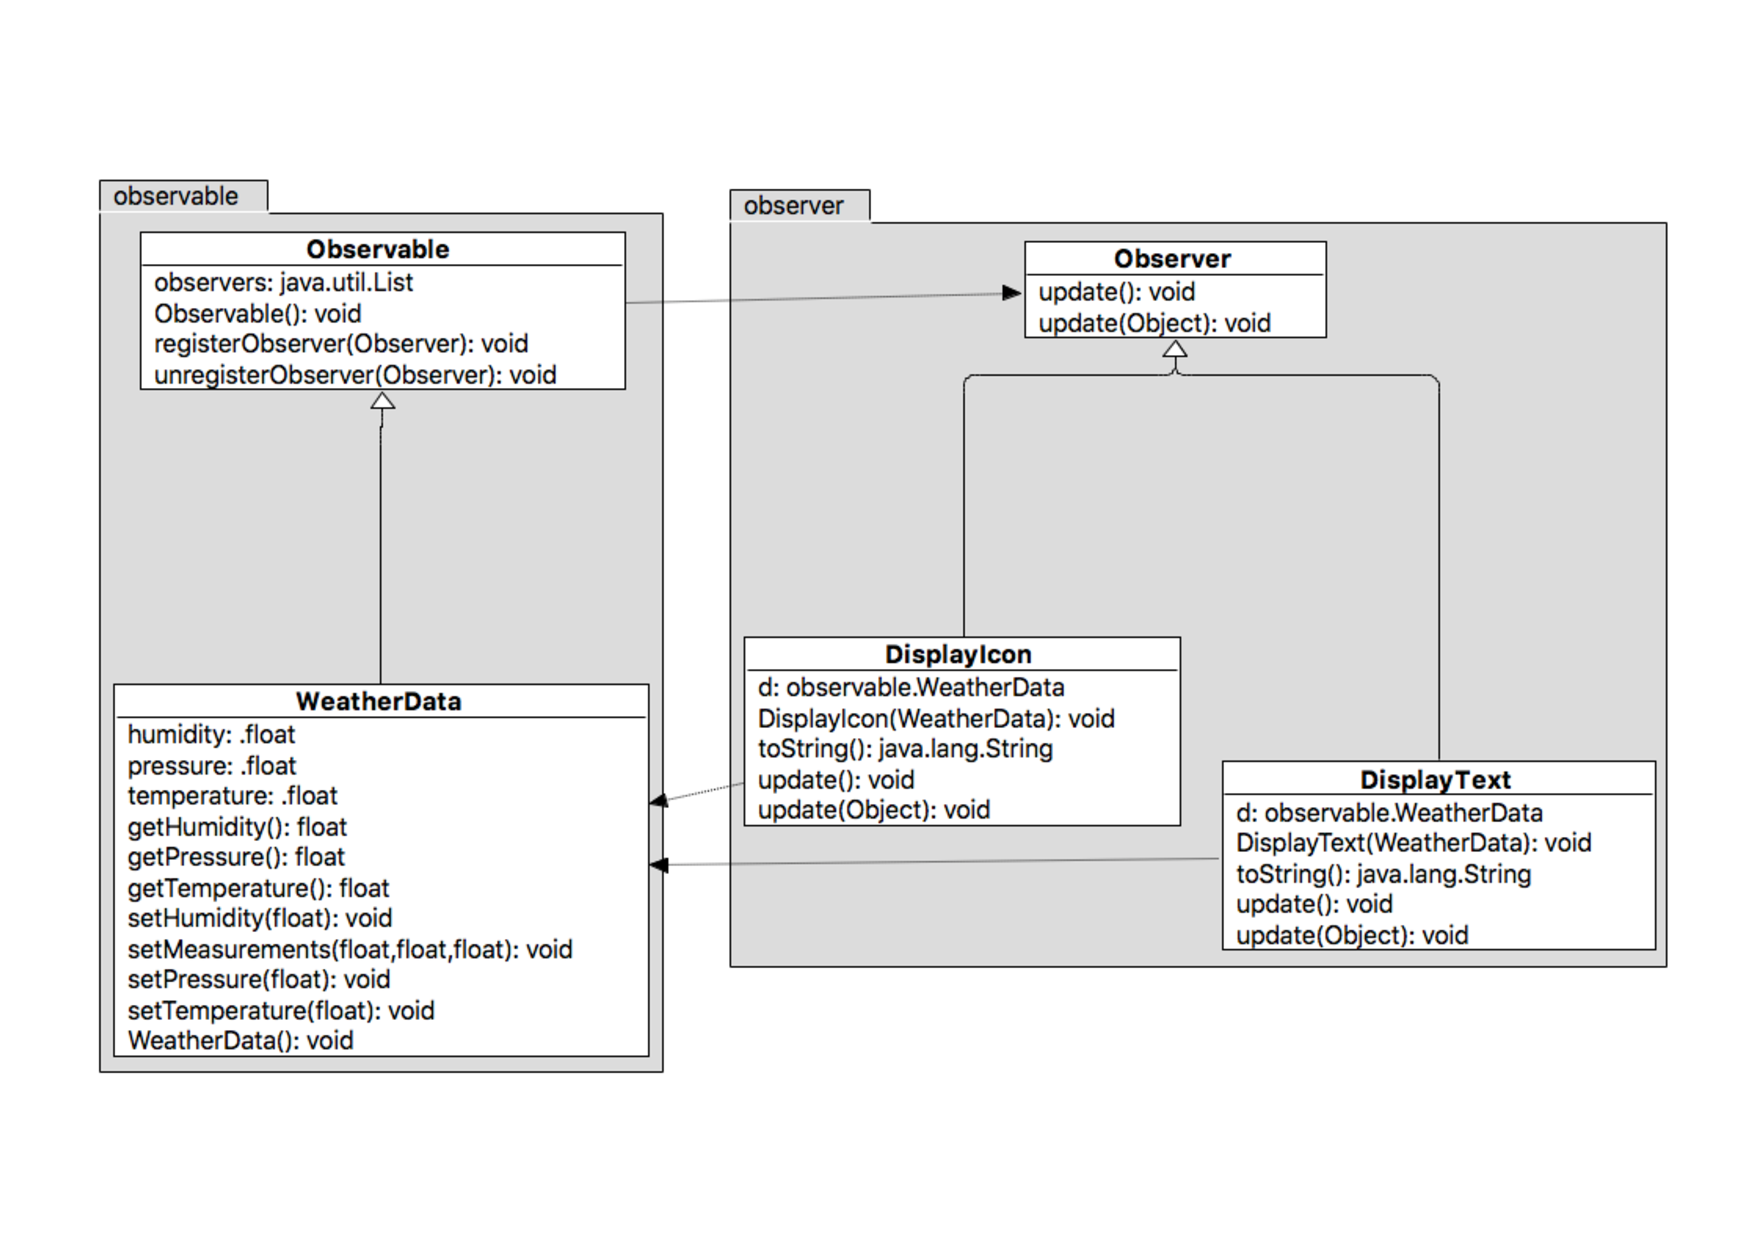
\includegraphics[width=1\textwidth]{Img/ObserverEsercizio5.pdf}
\caption{Class Diagram relativo alla soluzione dell'esercizio 5. Il diagramma \`e stato generato partendo dal codice utilizzando il tool descritto in laboratorio. Per questo il diagramma \`e lievemente divers da quello presentato in Figura~\ref{Fig:ObserverConcepts}}
\label{Fig:observerImpl1}
\end{figure}

\begin{lstlisting}[language=Java]
package observable;
import java.util.ArrayList;
import java.util.List;

import observer.Observer;

public abstract class Observable {

	private List<Observer> observers;
	
	public Observable(){
		observers=new ArrayList<Observer>();
	}
	
	public void registerObserver(Observer o){
		observers.add(o);
	}
	
	public void unregisterObserver(Observer o){
		this.observers.remove(o);
	}
	
	public void notifyObservers(){
		for(Observer o: this.observers){
			o.update();
		}
	}
	public <C> void notifyObservers(C c){
		for(Observer o: this.observers){
			o.update(c);
		}
	}	
}
\end{lstlisting}

\begin{lstlisting}[language=Java]
package observable;

public class WeatherData extends Observable {
	private float temperature;
	private float humidity;
	private float pressure;

	public WeatherData() {
		setTemperature(0);
		setHumidity(0);
		setPressure(1);
	}

	public void setMeasurements(float temperature, float humidity,
			float pressure) {
		this.humidity=humidity;
		this.temperature=temperature;
		this.pressure=pressure;
		this.notifyObservers();
	}

	public float getTemperature() {
		return temperature;
	}

	public void setTemperature(float temperature) {
		this.temperature = temperature;
		this.notifyObservers(temperature);
	}

	public float getHumidity() {
		return humidity;
	}

	public void setHumidity(float humidity) {
		this.humidity = humidity;
		this.notifyObservers(humidity);
	}

	public float getPressure() {
		return pressure;
	}

	public void setPressure(float pressure) {
		this.pressure = pressure;
		this.notifyObservers(pressure);
	}
}
\end{lstlisting}

\begin{lstlisting}[language=Java]
package observer;

public interface Observer {

	public void update();
	public <C> void update(C change);
}
\end{lstlisting}

\begin{lstlisting}[language=Java]
package observer;
import observable.WeatherData;

public class DisplayText implements Observer {

	private WeatherData d;

	public DisplayText(WeatherData d) {
		this.d = d;
		d.registerObserver(this);
	}

	public void update() {
		// o contiene l'oggetto osservabile che ha chiamato la notify
		// arg contiene dei parametri addizionali che possono essere passati
		// dall'oddetto osservato
		System.out.println(this.toString());

	}

	@Override
	public String toString() {
		return "WeatherData [temperature=" + d.getTemperature() + ", humidity="
				+ d.getHumidity() + ", pressure=" + d.getPressure() + "]";
	}

	public <C> void update(C change) {
		System.out.println("Text change: "+change);
		
	}
}
\end{lstlisting}
\begin{lstlisting}[language=Java]
package observer;

import observable.WeatherData;

public class DisplayIcon implements Observer {

	private WeatherData d;

	public DisplayIcon(WeatherData d) {
		this.d = d;
		d.registerObserver(this);
	}

	public void update() {
		// o contiene l'oggetto osservabile che ha chiamato la notify
		// arg contiene dei parametri addizionali che possono essere passati
		// dall'oddetto osservato

		System.out.println(this.toString());
	}
	
	public <C> void update(C change) {
		System.out.println("Icon change: "+change);
	}

	@Override
	public String toString() {
		if(d.getTemperature()>0)
			return "Icon: hot";
		return "Icon: cold";
	}	
}
\end{lstlisting}
\begin{lstlisting}[language=Java]
import observable.WeatherData;
import observer.DisplayIcon;
import observer.DisplayText;

public class Client {

	public static void main(String[] args) {
		WeatherData wd=new WeatherData();
		DisplayText dispText=new DisplayText(wd);
		DisplayIcon dispIcon=new DisplayIcon(wd);
		
		System.out.println(dispText.toString());
		System.out.println(dispIcon.toString());
		
		System.out.println("--------");
		wd.setMeasurements(10, 15, 20);
		
		System.out.println("--------");
		wd.setTemperature(30);
	}
}
\end{lstlisting}




\subsection{Iterator}
\begin{framed}
Supponendo che sia definita la classe:
\begin{lstlisting}[language=Java]
public class Matrix {
	
	public int rows(){
	    /**/
	}
	public int columns(){
    	/**/
	}
	public float element(int row, int column){/**/}
}
\end{lstlisting}
Si scriva in Java un opportuno iteratore che gestisca l’accesso sequenziale (per riga) agli elementi della matrice
\end{framed}
\begin{figure}[h]
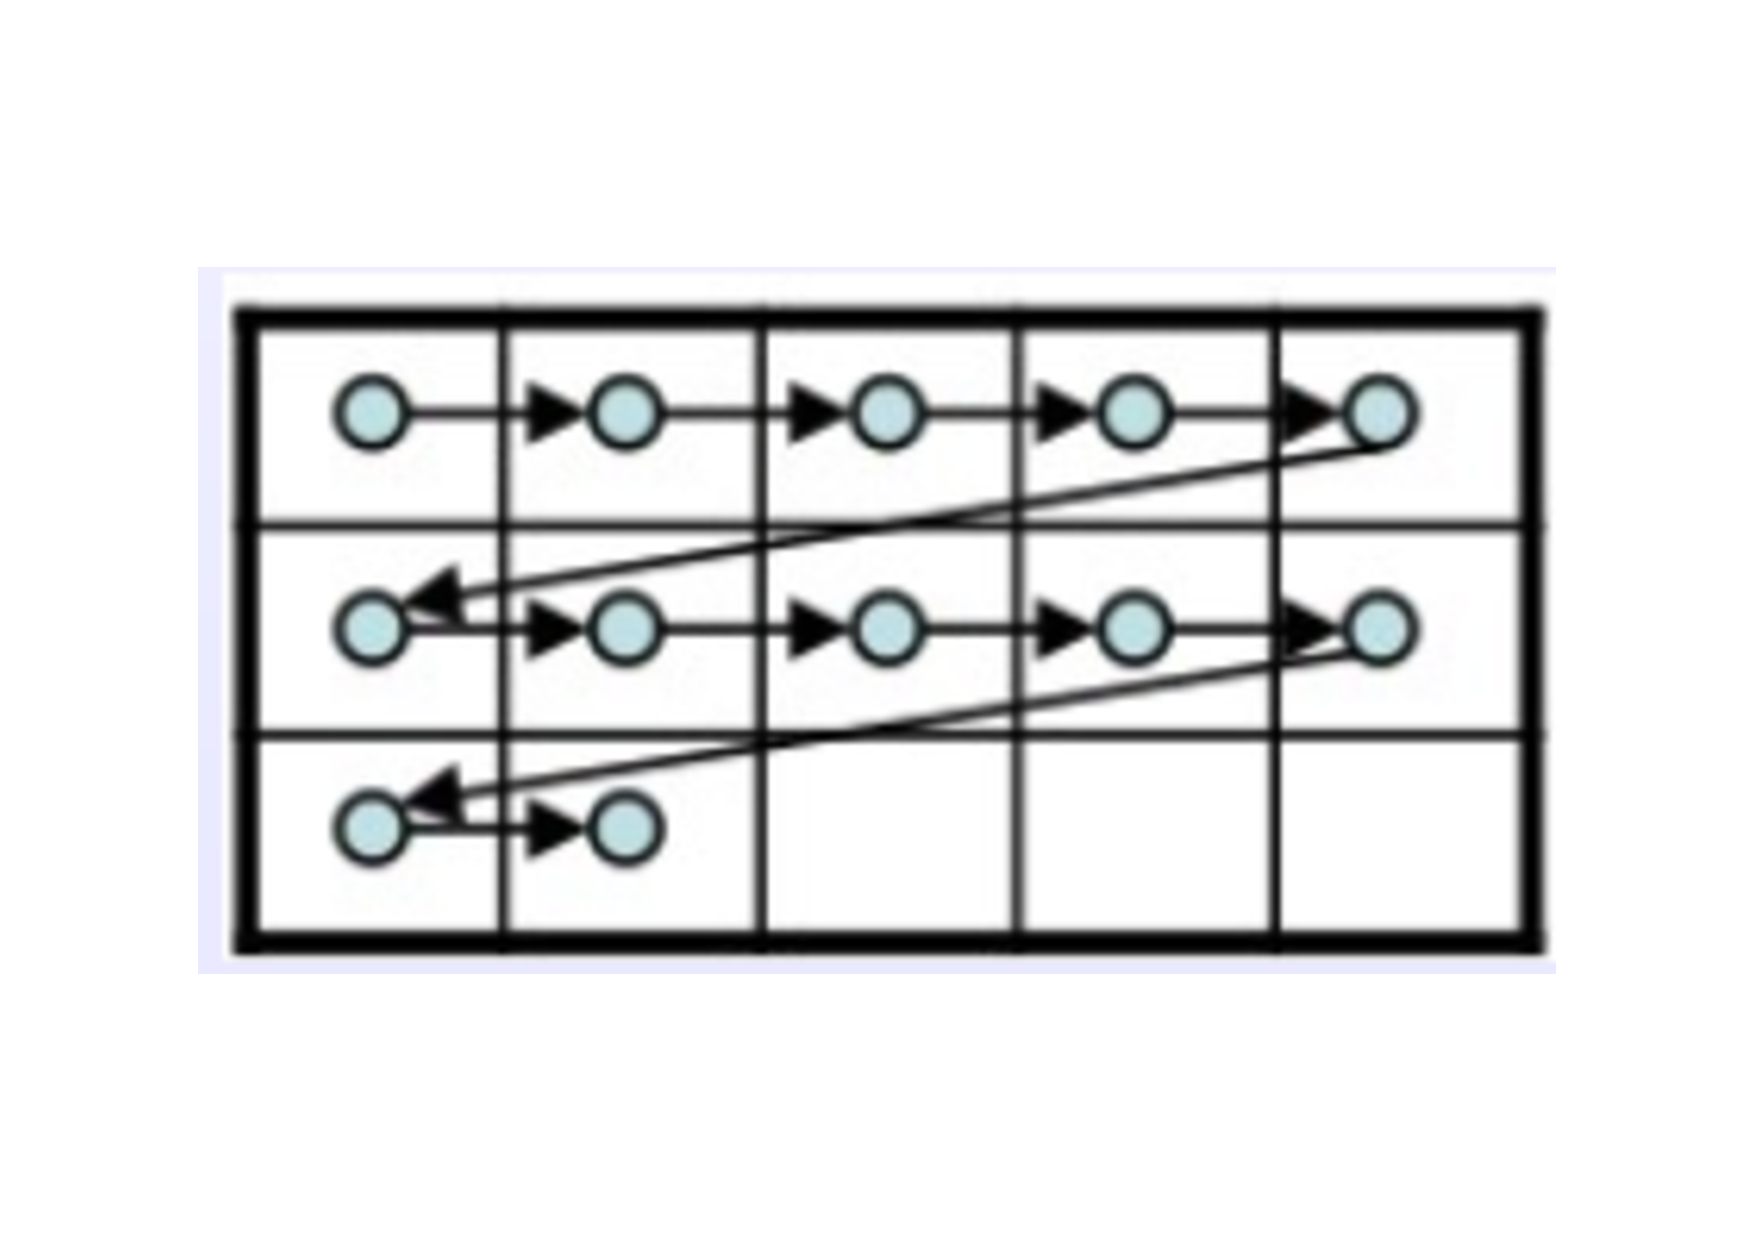
\includegraphics[width=0.4\textwidth]{Img/Matrix.pdf}
\end{figure}


\begin{lstlisting}[language=Java]
public class Matrix implements Iterable<Float>{
	// Iterable indica che la matrice deve essere iterabile questo implica che 
	// deve essere implementato il metodo  Iterator<Float> iterator() contenuto all'interno dell'
	// interfaccia Iterable
	private float[][] matrix;
	
	private int rows;
	
	private int columns;
	
	public Matrix(int rows, int columns) {
		this.rows = rows;
		this.columns = columns;
		matrix = new float[rows][columns];
	}
	
	public int rows(){
		return rows;
	}
	public int columns(){
		return columns;
	}
		
	public float element(int row, int column){
		return matrix[row-1][column-1];
	}
	
	public void setElement(int row, int column, float value){
		matrix[row-1][column-1] = value;
	}

	// passa al costruttore la matrice sulla quale si vuole iterare
	@Override
	public Iterator<Float> iterator() {
		return new MatrixIterator(this);
	}

	// classe interna. Viene dichiarata static visto che \`e associata alla classe non a un oggetto
	// IMPLEMENTA l'interfaccia iterator
	private static class MatrixIterator implements Iterator<Float> {
		// considerato che MatrixIterator implementa Iterator \`e necessario implementare
		// i corrispettivi metodi next, hasNext e remove
		private Matrix matrix;
		
		private int currentRow = 1;
		private int currentColumn = 1;
		
		public MatrixIterator(Matrix matrix) {
			this.matrix = matrix;
		}

		@Override
		public boolean hasNext() {
			return currentRow <= matrix.rows();
		}

		@Override
		public Float next() {		
			float element;
			try{
				element = matrix.element(currentRow, currentColumn);
			}catch(ArrayIndexOutOfBoundsException e){
				throw new NoSuchElementException();
			}
			currentColumn++;
			if(currentColumn>matrix.columns()){
				currentColumn = 1;
				currentRow++;
			}
			return element;
		}

		@Override
		public void remove() throws UnsupportedOperationException{
			throw new UnsupportedOperationException();		
		}
	}
}
\end{lstlisting}

\section{Esercizi per casa}
\begin{itemize}
\item Esercizi:
\begin{itemize}
\item La soluzione dell'esercizio 1 presenta delle inutili ripetizioni di codice, relativamente alla gestione dei messaggi e delle azioni. Pensare a come \`e possibile rimuoverle. Pensare e discutere (anche in forma testuale) o implementare possibili soluzioni.
\item Dove \`e possibile applicare il proxy pattern nell'esempio degli scacchi?  Pensare e discutere (anche in forma testuale) o implementare una possibile soluzione
\item \`E necessarial ka dichiarazione di \texttt{private WeatherData d;} in DisplayIcon e DisplayText all'interno della seconda implementazione dell'Observer?
\end{itemize} 
\end{itemize}




\clearpage

% ---- Bibliography ----




\addcontentsline{toc}{chapter}{Bibliography}
\bibliographystyle{alpha}
\bibliography{bib}
\nocite{*}


\end{document}

